\chapter{Progettazione e codifica}
\label{cap:progettazione-codifica}

\section{Tecnologie e strumenti}
\label{sec:tecnologie-strumenti}

In questa sezione, si descrivono le tecnologie utilizzate sia per ENGaming sia per i giochi.
Infatti, nonostante i giochi non necessitino di modifiche per il funzionamento in ENGaming, trovo comunque opportuno citarne le tecnologie che utilizzano, che ritengo possano essere interessanti.

\subsection{Tecnologie e strumenti del prodotto}

\subsubsection{Electron}
\begin{figure}[h]
    \centering
    
\includegraphics[width=150pt]{images/technologies/electron.png}
    \caption{Logo di Electron}
    \label{fig:electron}
\end{figure}
\gls{elctr} viene utilizzato per creare l'applicazione desktop, visualizzandola nello schermo dell'ENSign11.
Inoltre, si occupa della comunicazione tra il backend e il frontend dell'applicazione, attraverso canali di \gls{ipcg}.
\newpage
\subsubsection{Angular}
\label{subsec:angular}
\begin{figure}[h]
    \centering
    
\includegraphics[width=150pt]{images/technologies/angular.png}
    \caption{Logo di Angular}
    \label{fig:angular}
\end{figure}
\gls{angl} è il framework scelto per la realizzazione della parte visiva dell'applicazione.
Angular permette la creazione di Componenti, ovvero di elementi o pagine, dove sono presenti:
\begin{itemize}
    \item un file \gls{html}, per la visualizzazione del componente;
    \item un foglio di stile (\gls{css}/SASS/LESS) per gli effetti grafici;
    \item un file \gls{tsc}, per definire il comportamento del componente.
\end{itemize}
Inoltre, permette l'utilizzo di Servizi per il trasferimento di dati tra componenti.
\subsubsection{TypeScript}
\begin{figure}[h]
    \centering
    
\includegraphics[width=150pt]{images/technologies/typescript.png}
    \caption{Logo di TypeScript}
    \label{fig:typescript}
\end{figure}
\gls{tsc} viene utilizzato sia da Electron che da Angular (da quest'ultimo per la definizione del comportamento di componenti e servizi).
Ciò che caratterizza \gls{tsc} da \gls{js} è la tipizzazione delle variabili, elemento che trovo molto utile sopratutto se si è in precedenza lavorato con linguaggi di programmazione come Java e C++, come nel mio caso.
I sorgenti scritti in questo linguaggio devono poi essere compilati per generare il file \gls{js} effettivamente letto dal browser.

\subsubsection{C++}
\begin{figure}[h]
    \centering
    
\includegraphics[width=150pt]{images/technologies/cpp.png}
    \caption{Logo di C++}
    \label{fig:cpp}
\end{figure}
\gls{cpp} è utilizzato per la logica relativa al device. In particolare, attraverso un driver (fornito dall'azienda), si possono rilevare le interazioni con il device (sia tramite tocco che tramite digitalizer).

\subsubsection{Node-API}
\begin{figure}[h]
    \centering
    
\includegraphics[width=150pt]{images/technologies/nodeapi.png}
    \caption{Logo delle Node-API}
    \label{fig:nodeapi}
\end{figure}
Le \gls{napi} sono utilizzate per rendere la parte in C++ "usabile" dalla parte sviluppata in Electron.
Infatti, senza di esse, non sarebbe possibile utilizzare i metodi per l'interazione con il device.

\subsubsection{Electron-Forge}
\gls{elctrForge} viene utilizzato per creare degli installer, o dei pacchetti, a seconda del sistema operativo in cui si va a compilare il progetto.
Tale strumento permette di compilare l'applicazione per Windows, Linux e MacOS, e ciò permette di definire ENGaming come un applicativo multipiattaforma.
\newpage
\subsection{Tecnologie e strumenti dei giochi}

\subsubsection{HTML-CSS-JavaScript}
\begin{figure}[h]
    \centering
    
\includegraphics[width=300pt]{images/technologies/HTMLCSSJS.png}
    \caption{Loghi di HTML, CSS e JavaScript}
    \label{fig:HTMLCSSJS}
\end{figure}
I giochi che ENGaming esegue sono semplici giochi eseguibili anche su browser. Per tale motivo, sono scritti con \gls{html} per la struttura (generalmente composta da canvas), \gls{css} per lo stile e \gls{js} per il gioco vero e proprio.
Per usufruire al meglio di tutte le funzionalità che l'applicativo offre, in particolare per poter salvare i record relativi ai giochi, è necessario che i giochi stessi implementino una piccola modifica, che consiste nell'inviare un messaggio all'applicativo.
Infatti, essendo il gioco visualizzato all'interno di una pagina (attraverso un elemento iframe), è necessario che il gioco mandi il punteggio "in alto", utilizzando la seguente riga di codice:
\begin{lstlisting}
    window.top.postMessage({type:'gameIsOver',data:score});
\end{lstlisting}
Questo comando manda un messaggio con il punteggio conseguito. Il tipo (in questo caso, "gameIsOver") indica la tipologia del messaggio, in modo da poterlo distinguere rispetto ad altri messaggi.
\newpage
\subsubsection{WebAssembly}
\begin{figure}[h]
    \centering
    
\includegraphics[width=150pt]{images/technologies/webassembly.png}
    \caption{Logo di WebAssembly}
    \label{fig:webassembly}
\end{figure}
Nel caso si volesse eseguire un classico nell'ENGaming (ad esempio, Doom), bisogna prima passare per \gls{webassembly}, in modo da renderlo eseguibile su un browser.
Le modifiche da fare per il funzionamento dipendono dal singolo gioco, è in ogni caso indispensabile essere in possesso dei sorgenti.
Tale gioco viene poi letto da un normale file \gls{js} attraverso il file con estensione .wasm, che non permette di effettuare la modifica per la ricezione del punteggio, quindi per tali giochi non si possono avere record salvati.

\section{Progettazione}
\label{sec:progettazione}
\subsection{Classi utilizzate}
\begin{figure}[h]
    \centering
    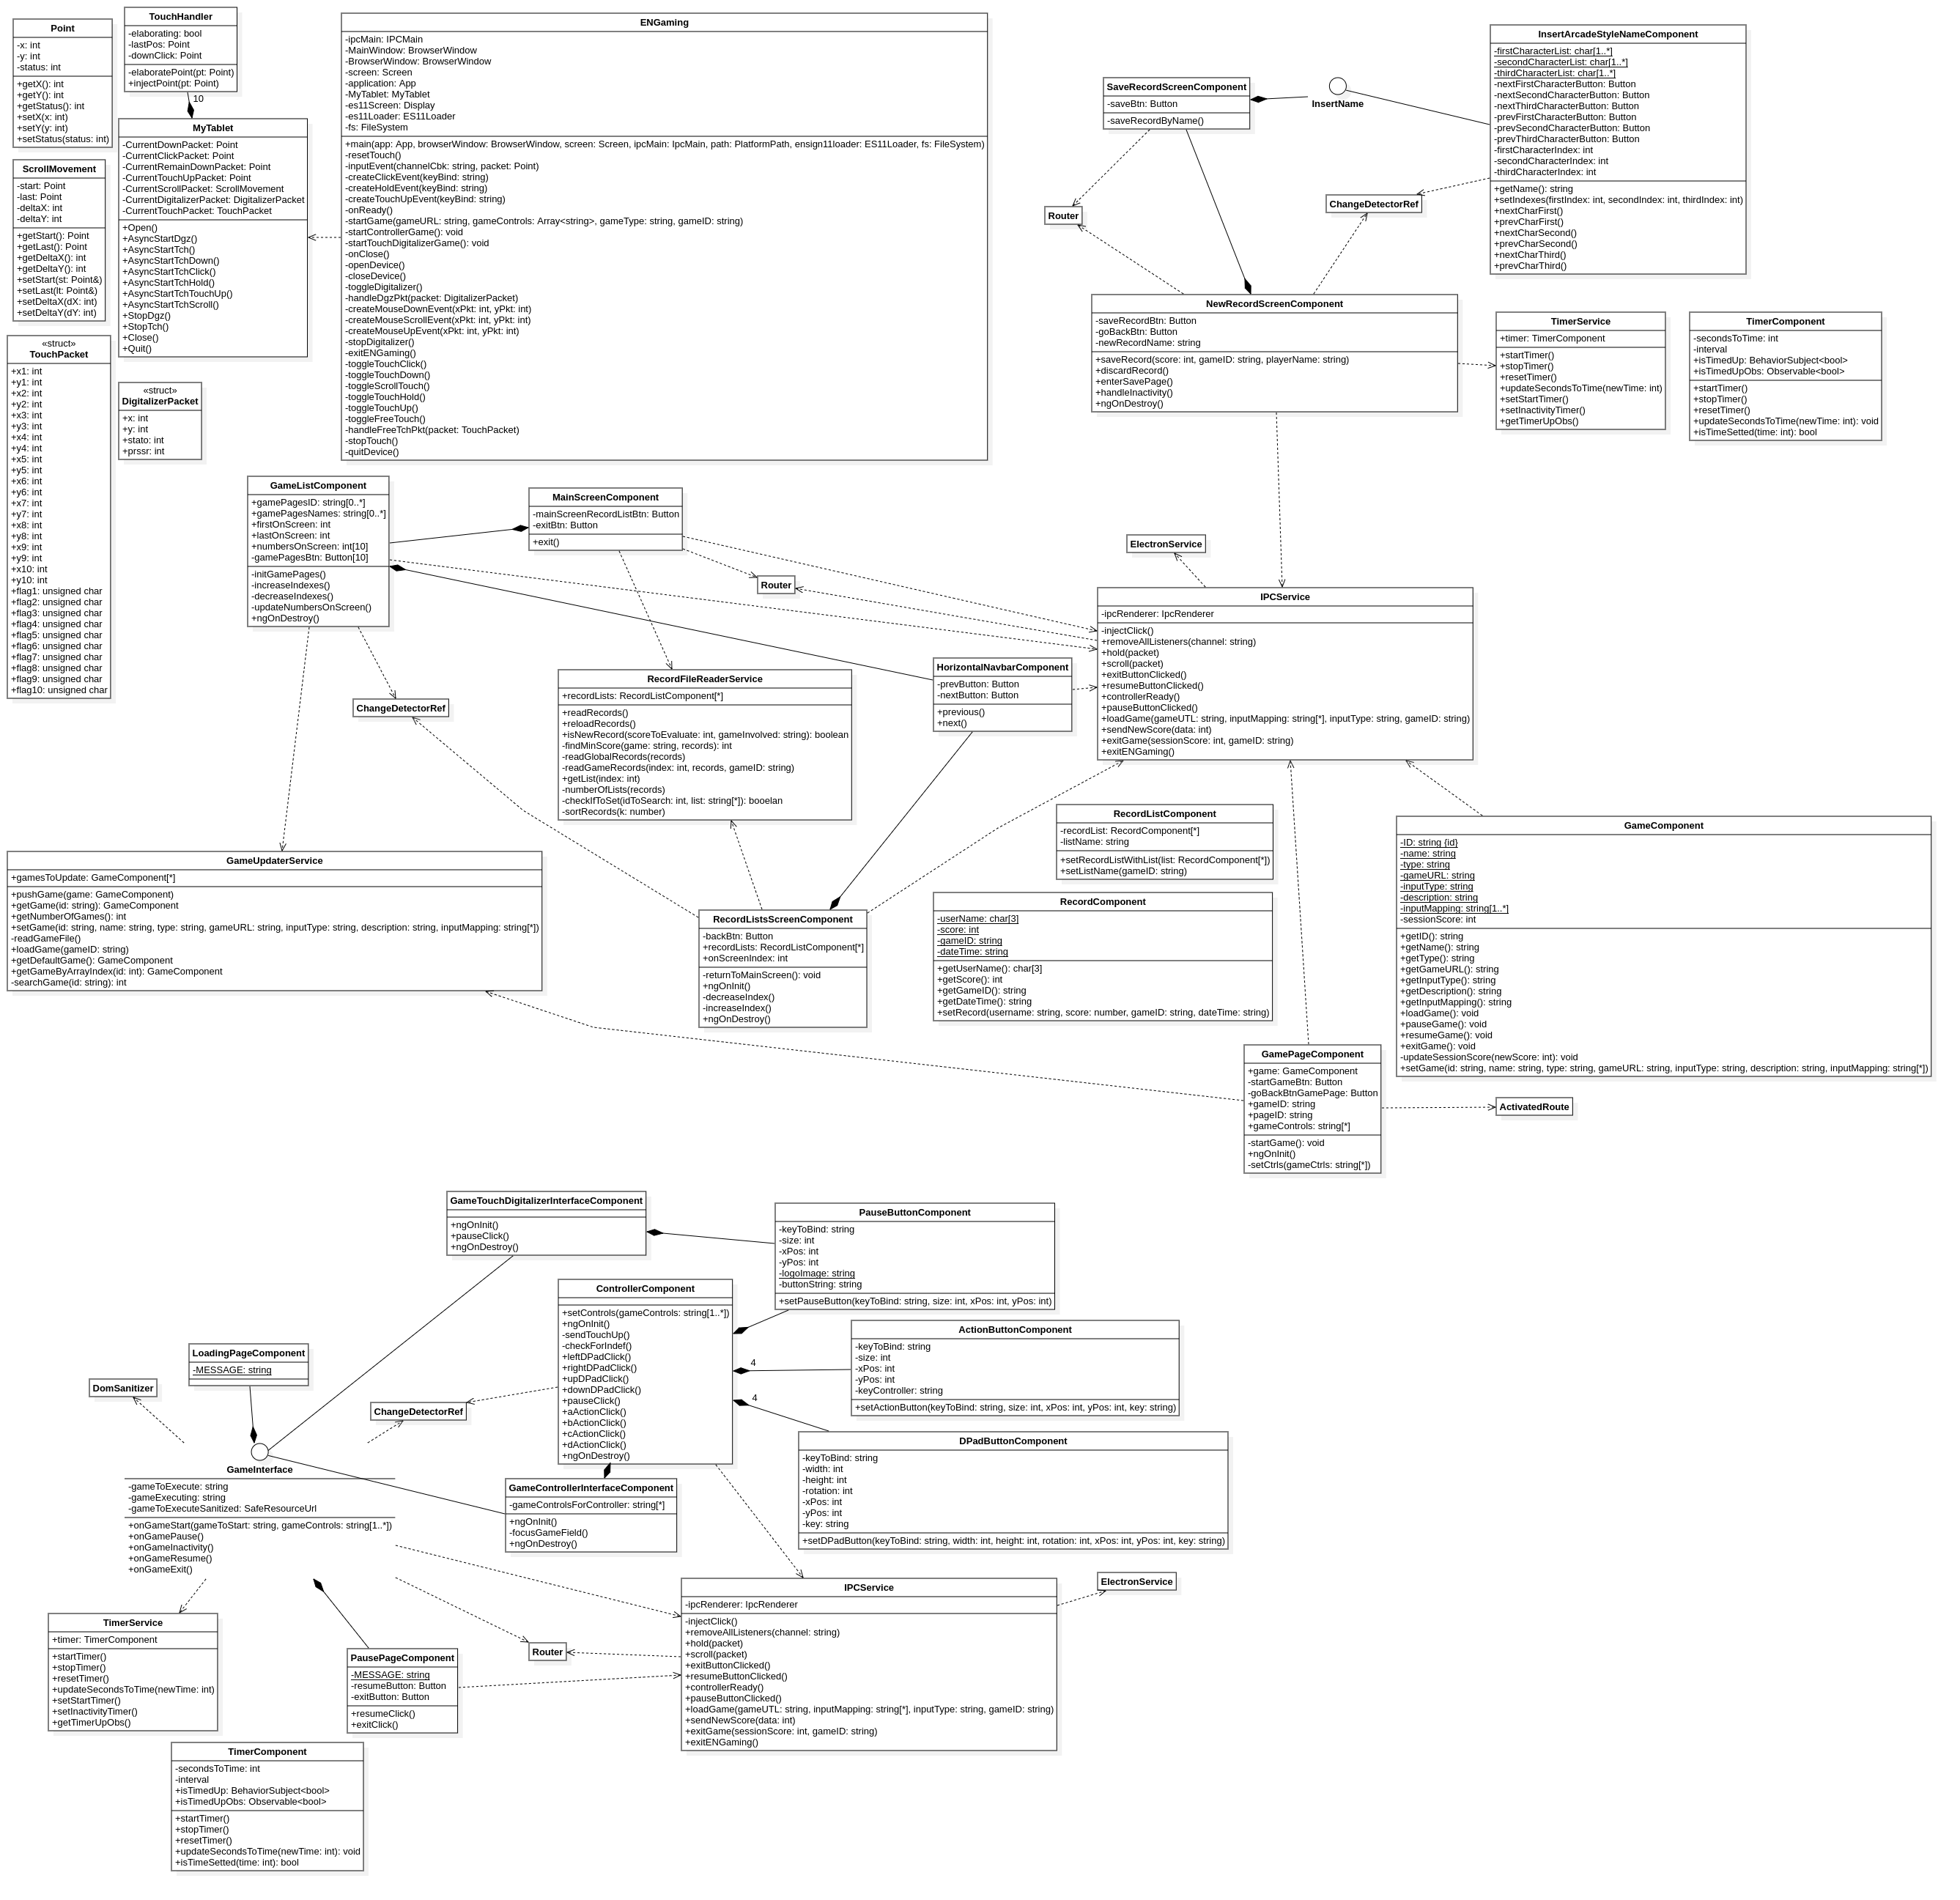
\includegraphics[width=340pt]{images/prog/ENGaming.png}
    \caption{Diagramma completo delle classi utilizzate}
    \label{fig:diagrammaCompleto}
\end{figure}
% immagine grafico completo
Le classi utilizzate possono essere classificate tramite il linguaggio d'implementazione:
\begin{itemize}
    \item Electron: \begin{itemize}
        \item ENGaming
    \end{itemize}
    \item C++: \begin{itemize}
        \item MyTablet
        \item TouchHandler
        \item Point
        \item ScrollMovement
        \item TouchPacket
        \item DigitalizerPacket
    \end{itemize}
    \item Angular: \begin{itemize}
        \item Tutte le classi "Component"
        \item Tutte le classi "Service"
        \item GameInterface
        \item InsertName
        \item Router
        \item ChangeDetectorRef
        \item DomSanitizer
        \item ActivatedRoute
    \end{itemize}
\end{itemize}
Di seguito si analizzano le vari componenti con maggior dettaglio.
\newpage
\subsubsection{ENGaming}
\begin{figure}[h]
    \centering
    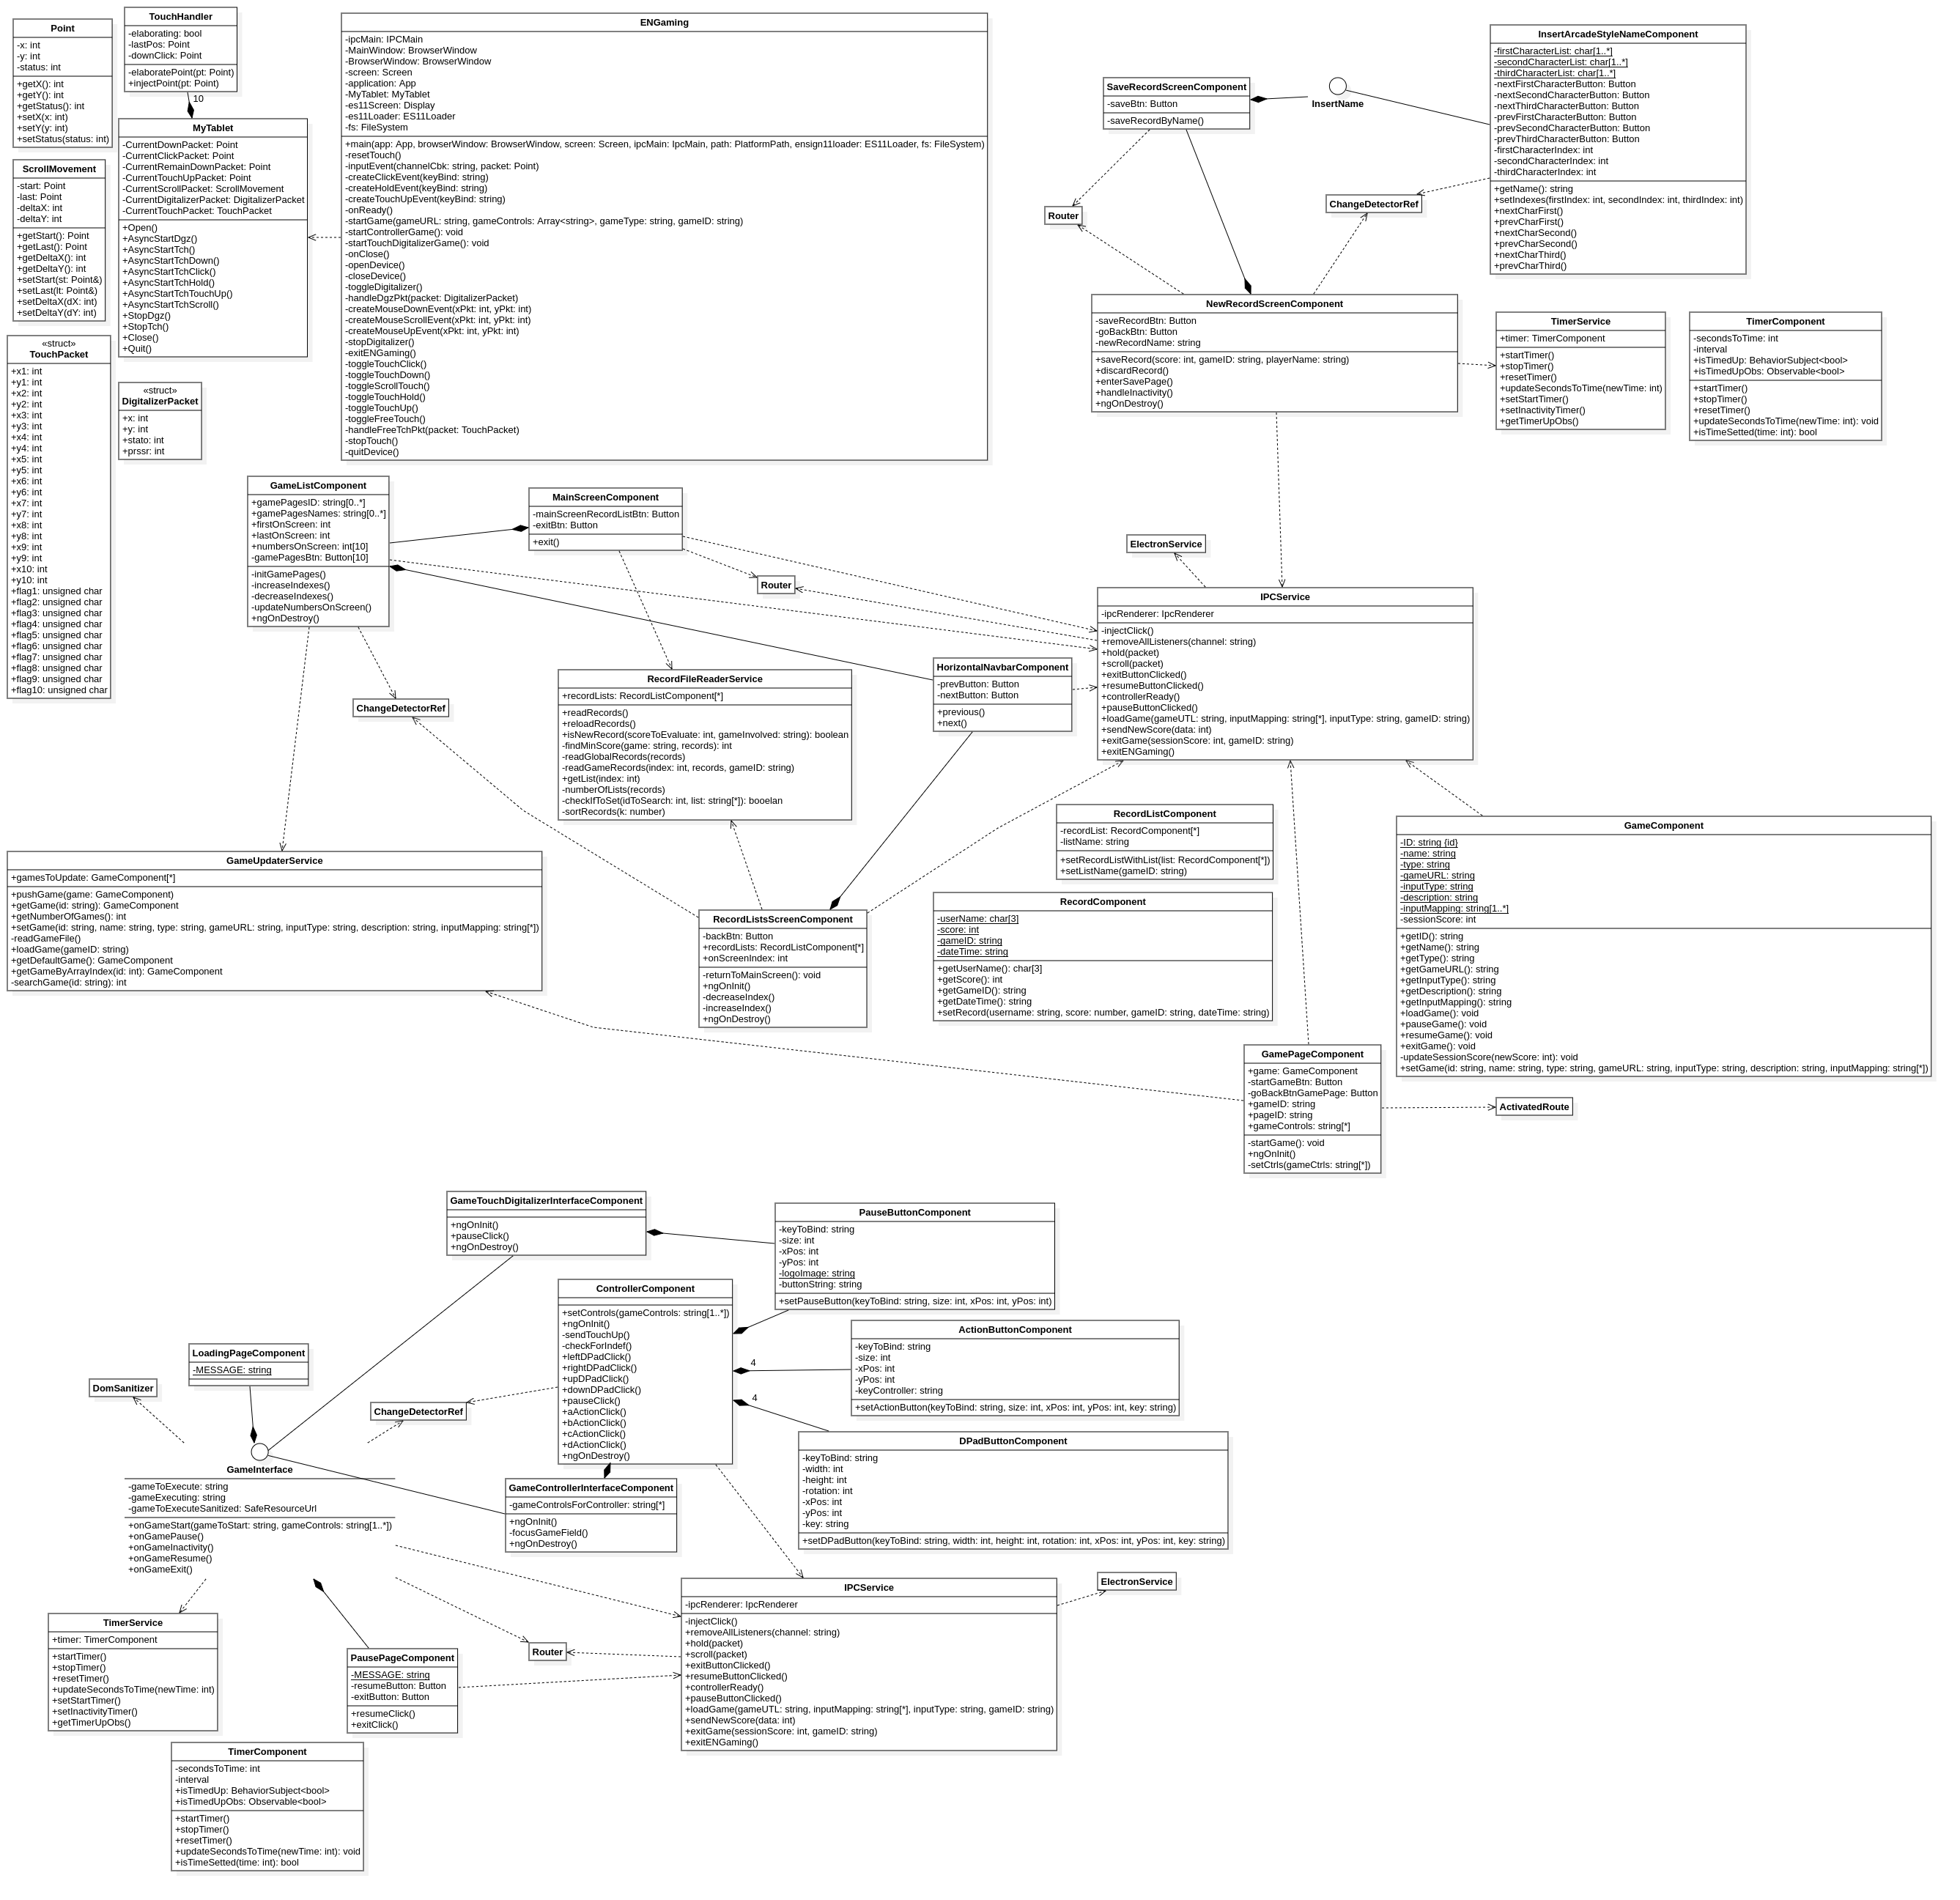
\includegraphics[width=340pt]{images/prog/ENGaming.png}
    \caption{Classe ENGaming}
    \label{fig:engaming}
\end{figure}
% immagine dettaglio ENGaming
La classe \emph{ENGaming} si occupa dell'avvio dell'applicazione.\\ Sviluppata in \gls{elctr}, contiene i componenti necessari per la creazione della finestra nell'ENSign 11 (Screen, BrowserWindow) e per la comunicazione con la parte in \gls{angl} (IPCMain).\\
Inoltre, contiene anche i moduli per la comunicazione con ENSign11.\\
Contiene:
\begin{itemize}
    \item i metodi per interagire con l'ENSign11: \begin{itemize}
        \item \emph{openDevice}, per aprire il device.
        \item \emph{toggleTouchClick}, per ricevere un click.
        \item \emph{toggleTouchDown}, per ricevere un down, ovvero l'evento di un dito appoggiato sullo schermo del device.
        \item \emph{toggleTouchHold}, per ricevere un hold, ovvero l'evento di un dito ancora appoggiato sullo schermo del device.
        \item \emph{toggleTouchUp}, per ricevere un touch up, ovvero l'evento di un dito sollevato dallo schermo del device.
        \item \emph{toggleScrollTouch}, per ricevere un evento di scroll, ovvero un evento di movimento di un dito sullo schermo del device.
        \item \emph{toggleFreeTouch}, per ricevere i pacchetti definiti nella struttura \emph{TouchPacket}.
        \item \emph{stopTouch}, per fermare le interazioni con lo schermo del device.
        \item \emph{toggleDigitalizer}, per ricevere i pacchetti definiti nella struttura \emph{DigitalizerPacket}.
        \item \emph{stopDigitalizer}, per fermare le interazioni con il digitalizer.
        \item \emph{closeDevice}, per chiudere il device.
        \item \emph{quitDevice}, per "liberare" il device e renderlo disponibile ad altri applicativi (o a una nuova istanza di ENGaming).
    \end{itemize}
    \item i metodi per l'avvio dei giochi: \begin{itemize}
        \item \emph{startGame}: identifica la tipologia del gioco e lo inizializza.
        \item \emph{startControllerGame}: inizializza un gioco che richiede l'uso del controller.
        \item \emph{startTouchDigitalizerGame}: inizializza un gioco che richiede l'uso del dito o del digitalizer.
    \end{itemize}
    \item i metodi per interagire con un gioco che utilizza il controller: \begin{itemize}
        \item \emph{inputEvent}, che permette l'interazione con il controller, nell'apposito componente.
        \item \emph{createClickEvent}, che crea l'evento "click" nella pagina del gioco.
        \item \emph{createHoldEvent}, che crea l'evento "hold" nella pagina del gioco.
        \item \emph{createTouchUpEvent}, che crea l'evento "touch up" nella pagina del gioco.
    \end{itemize}
    \item i metodi per interagire con un gioco che utilizza il dito o il digitalizer: \begin{itemize}
        \item \emph{handleFreeTchPkt}: in base allo stato del pacchetto, si decide che evento sollevare.
        \item \emph{handleDgzPkt}: come per \emph{handleFreeTchPkt}, per il digitalizer.
        \item \emph{createMouseDownEvent}: crea l'evento di appoggio del dito/digitalizer nel gioco.
        \item \emph{createMouseScrollEvent}, crea l'evento di movimento del dito/digitalizer nel gioco.
        \item \emph{createMouseUpEvent}, crea l'evento di sollevamento del dito/digitalizer nel gioco.
    \end{itemize}
    \item \emph{resetTouch}: ripristina il touch del device alla fine di un gioco.
    \item \emph{exitENGaming}: chiude l'applicazione.
\end{itemize}
\newpage
\subsubsection{Schermata iniziale}
\begin{figure}[h]
    \centering
    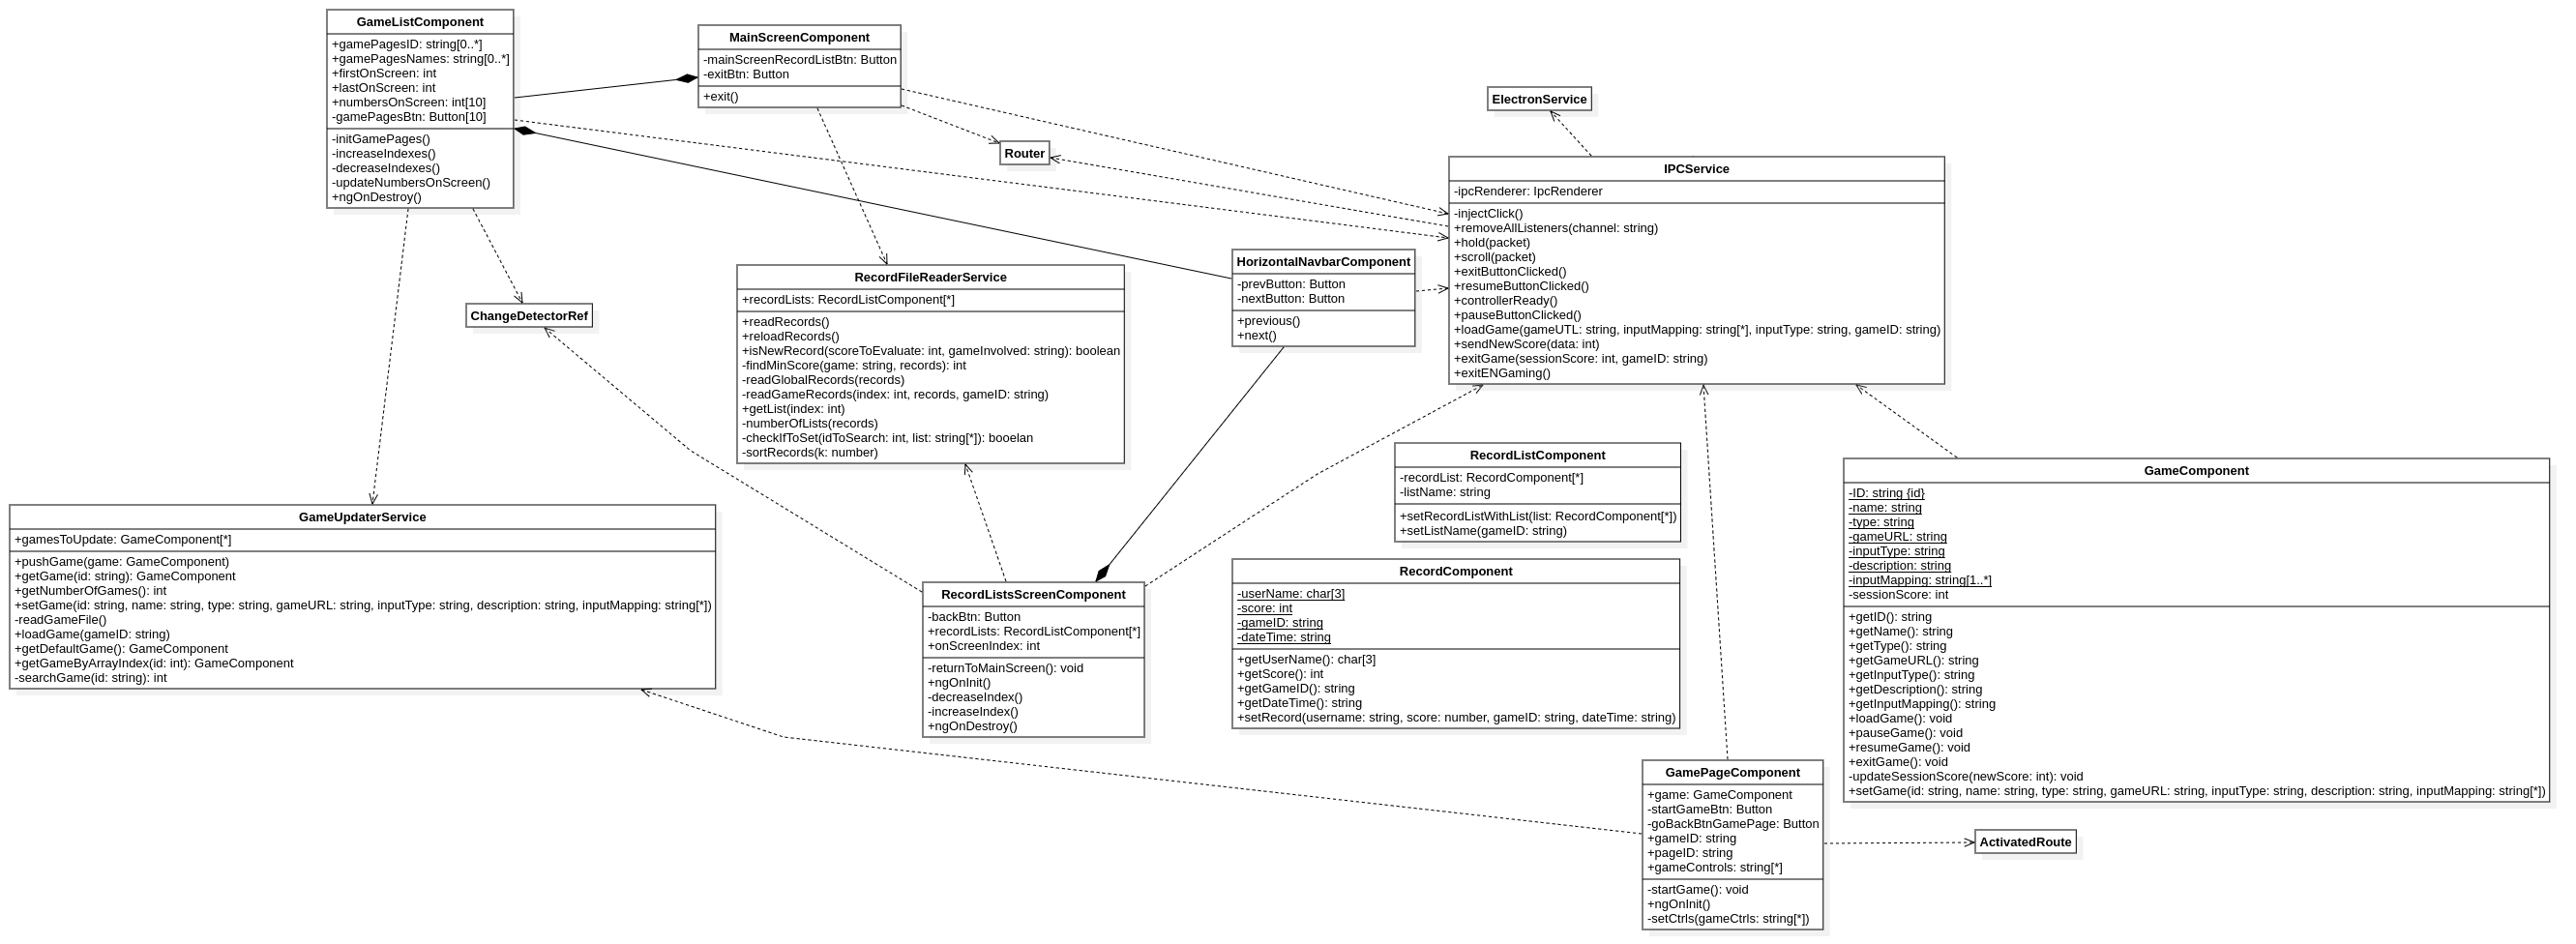
\includegraphics[width=340pt]{images/prog/MainScreen.png}
    \caption{Classi della schermata iniziale}
    \label{fig:schermataIniziale}
\end{figure}
% immagine dettaglio schermata iniziale
All'avvio dell'applicazione, la schermata iniziale presenta tre elementi:
\begin{itemize}
    \item L'elenco dei giochi disponibili, ottenuto da \emph{GameListComponent}.
    \item Il pulsante per accedere alla pagina di \emph{RecordListScreenComponent}.
    \item Il pulsante per uscire dall'applicazione.
\end{itemize}
Inoltre, il componente che gestisce questa schermata, ovvero \emph{MainScreenComponent}, si serve del service \emph{IPCService} per le comunicazioni attraverso le altre componenti dell'applicazione, utilizzando i canali IPC.
A sua volta:
\begin{itemize}
    \item \emph{RecordListScreenComponent} è formato da almeno un \emph{RecordListComponent}, poichè la schermata ha almeno la lista globale dei record. Inoltre, utilizza il \emph{HorizontalNavbarComponent} per navigare tra una lista e l'altra.
    \item \emph{RecordListComponent} contiene il nome della lista stessa e utilizza \emph{IPCService} per la comunicazione con il resto dell'applicazione.\\ Ovviamente, contiene anche vari \emph{RecordComponent}.
    \item \emph{GameListComponent} è formato sia dall' \emph{HorizontalNavbarComponent},\\ poichè gestisce la visualizzazione della lista di giochi disponibili, sia da almeno una \emph{GamePageComponent}, ossia da almeno una pagina relativa a un gioco.
    \item Ogni \emph{GamePageComponent} è relativa a un solo \emph{GameComponent}, le cui informazioni sono caricate da GameUpdaterService. Contiene sia il \emph{GameComponent}, sia i pulsanti per avviare il gioco e per tornare alla schermata principale.
\end{itemize}
\emph{GameComponent} e \emph{RecordComponent} utilizzano anche determinate proprietà, che si elencano negli appositi paragrafi rispettivamente in \nameref{subsec:gameComponent} e \nameref{subsec:recordComponent}.
\newpage
\subsubsection{GameComponent}
\label{subsec:gameComponent}
\begin{figure}[h]
    \centering
    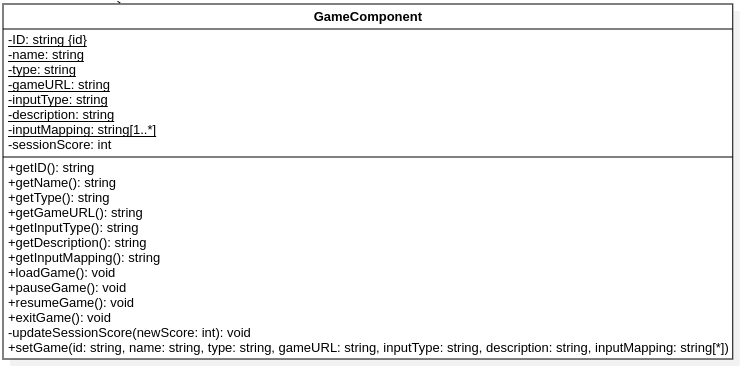
\includegraphics[width=340pt]{images/prog/Game.png}
    \caption{Dettaglio della classe GameComponent}
    \label{fig:gameComponent}
\end{figure}
% immagine dettaglio GameComponent
\emph{GameComponent} rappresenta un gioco all'interno dell'applicativo. Contiene tutte le informazioni necessarie per l'avvio e il controllo dello stesso, oltre alle classiche informazioni "anagrafiche".\\
Un gioco viene rappresentato come:
\begin{itemize}
    \item ID: l'identificativo del gioco, formato da una stringa.
    \item name: nome del gioco.
    \item type: la categoria del gioco.
    \item gameURL: l'indirizzo dove reperire la finestra di gioco, sia locale che remoto.
    \item inputType: la tipologia d'input, tra "controller" e "touchDigit" (ovvero touch/digitalizer).
    \item description: opzionale. Descrizione del gioco, con informazioni generali in merito. Se non sono disponibili, il campo assume valore "not_available".
    \item inputMapping: la mappatura dei controlli da utilizzare per giocare.
\end{itemize}
Inoltre, utilizza \emph{IPCService} per inviare e ricevere eventi inerenti al gioco in esecuzione, e utilizza la variabile sessionScore per registrare il punteggio di gioco più alto durante la sessione.
Infine, i giochi sono memorizzati nel file \emph{games.json}, della cui struttura si parlerà in \nameref{subsec:strutturaFile}. 
\subsubsection{RecordComponent}
\label{subsec:recordComponent}
\begin{figure}[h]
    \centering
    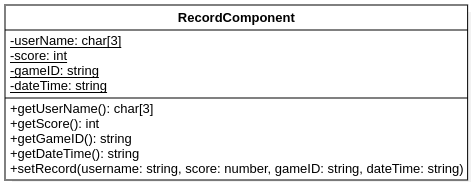
\includegraphics[width=340pt]{images/prog/Record.png}
    \caption{Dettaglio della classe RecordComponent}
    \label{fig:recordComponent}
\end{figure}
% immagine dettaglio RecordComponent
RecordComponent rappresenta un record memorizzato dall'applicativo.\\ Contiene le informazioni relative a un punteggio, effettuato da un determinato utente in un determinato gioco.\\
Un record viene rappresentato come:
\begin{itemize}
    \item userName: il nome dell'utente che ha effettuato un record, formato da un array di tre caratteri.
    \item score: il punteggio eseguito dall'utente.
    \item gameID: l'ID del gioco dove si è effettuato il record.
    \item dateTime: la data e ora di conseguimento del record.
\end{itemize}
I record sono memorizzati nel file \emph{records.json}, della cui struttura si parlerà sempre in \nameref{subsec:strutturaFile}.
\subsubsection{Interfaccia di gioco}
\begin{figure}[h]
    \centering
    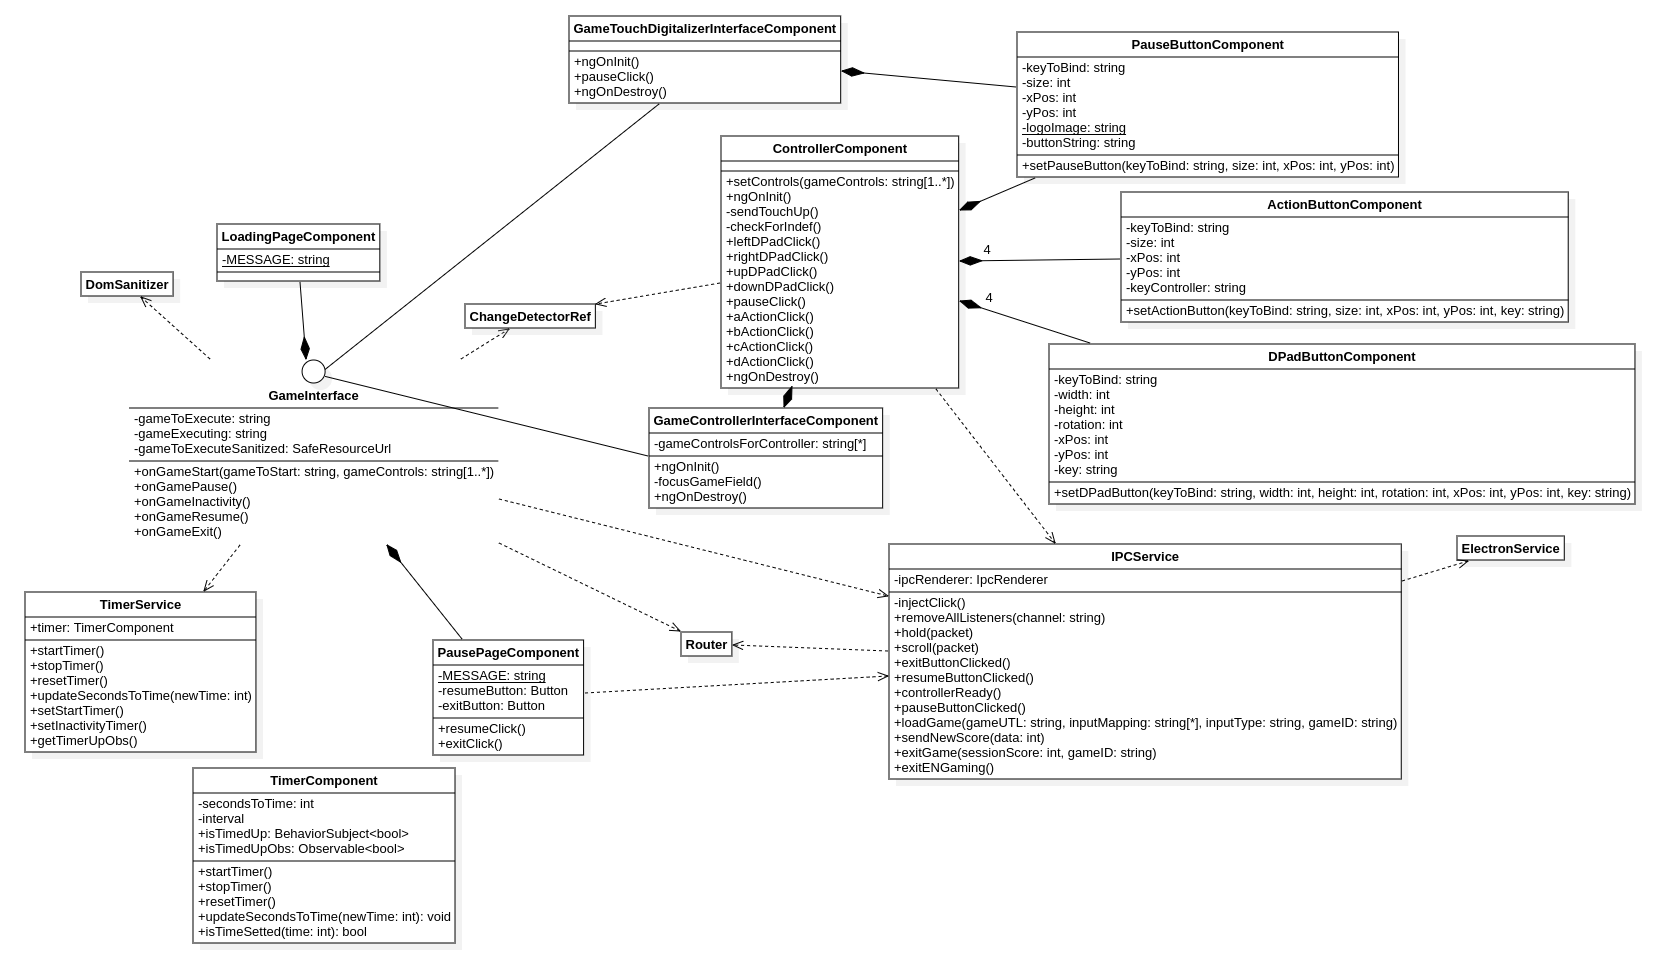
\includegraphics[width=340pt]{images/prog/GameInterface.png}
    \caption{Diagramma delle classi per l'interfaccia di gioco}
    \label{fig:gameinterface}
\end{figure}
% immagine dettaglio Interfaccia di gioco
Dovendo implementare due tipologie di gioco, dev'essere necessario poter creare due interfacce separate, che abbiano però elementi in comune.\\
Per questo motivo, viene utilizzata l'interfaccia \emph{GameInterface}, che contiene il necessario per la corretta visualizzazione del gioco.\\
In particolare, utilizza:
\begin{itemize}
    \item \emph{TimerComponent}, attraverso \emph{TimerService}, per la gestione della schermata di caricamento e lo stato d'inattività.
    \item \emph{LoadingPageComponent} per la visualizzazione della schermata di caricamento.
    \item \emph{PausePageComponent} per visualizzare l'informazione dello stato di pausa del gioco, con le possibilità di riprenderlo o di uscire dallo stesso.
    \item \emph{IPCService} per le comunicazioni tra componenti.
    \item \emph{Router}, \emph{DomSanitizer} e \emph{ChangeDetectorRef}, per i motivi elencati in \nameref{subsec:angularServices}.
\end{itemize}
Questa interfaccia viene implementata da due classi: \emph{GameControllerInterfaceComponent} e \emph{GameTouchDigitalizerInterfaceComponent}.
\newpage
\paragraph{GameControllerInterfaceComponent}
\label{paragraph:gamecontrollerinterfacecomponent}
\emph{GameControllerInterfaceComponent} rappresenta l'interfaccia di gioco per giochi che richiedono l'utilizzo del controller.\\
Questa classe, oltre a essere formata dagli elementi che implementa da \emph{GameInterface}, è formata da un controller. Il controller è composto da:
\begin{itemize}
    \item Quattro \emph{DPadButtonComponent}, che rappresentano i pulsanti per il movimento all'interno del gioco.
    \item Quattro \emph{ActionButtonComponent}, che rappresentano i pulsanti per le azioni\\ all'interno del gioco.
    \item Un \emph{PauseButtonComponent} per mettere in pausa il gioco.
\end{itemize}
Il controller viene configurato, prima dell'avvio, secondo i comandi previsti per il singolo gioco. Se uno o più pulsanti non vengono configurati per un determinato gioco, essi vengono rimossi dalla visualizzazione, al fine di non creare confusione durante l'utilizzo del gioco.\\
Infine, essendo il device target posizionato in un determinato modo, il layout è configurato in maniera da facilitarne l'utilizzo senza prendere in mano il device.\\
In particolare, gli \emph{ActionButtonComponent} presenti sono posizionati in modo da risultare il più possibilmente comodi per questa posizione, ispirandosi alla posizione della mano destra di un pianista.
Un layout di esempio, adatto per questi vincoli, è nell'immagine seguente:
\begin{figure}[h]
    \centering
    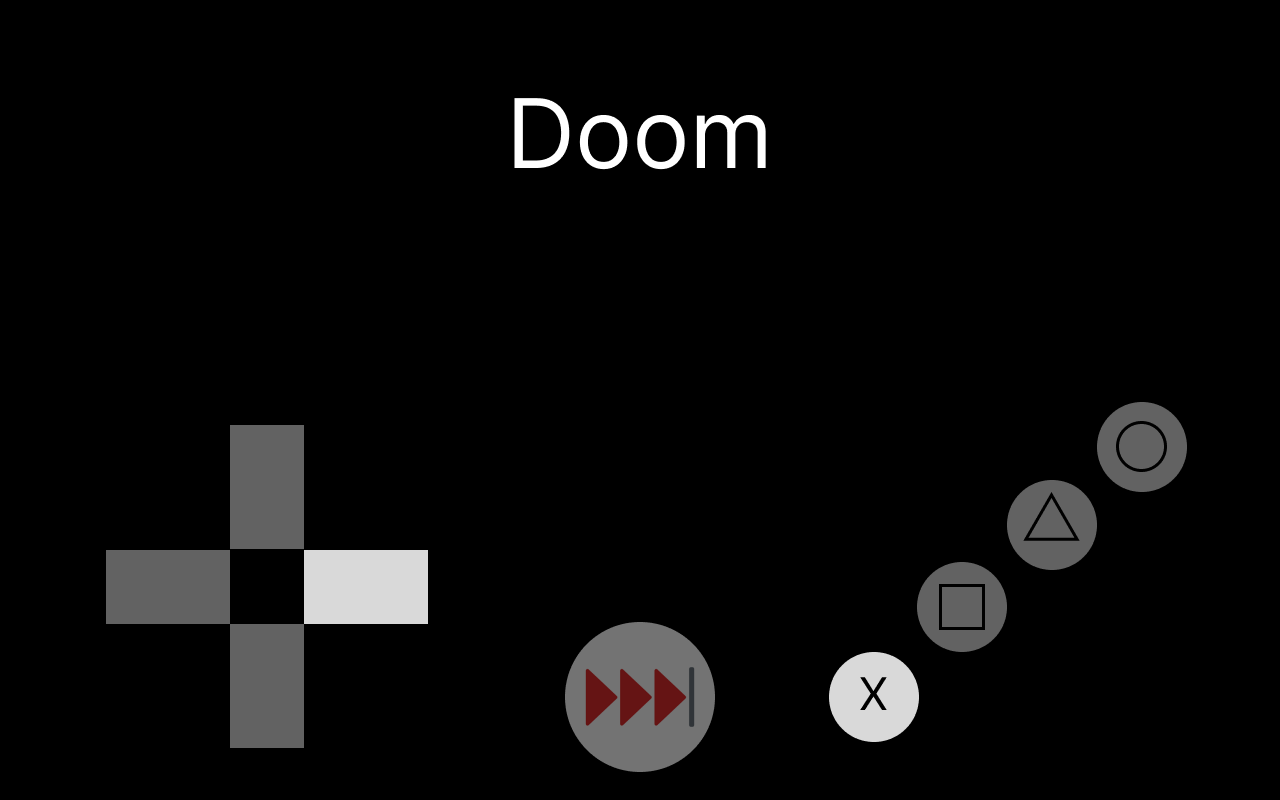
\includegraphics[width=340pt]{images/prog/ControllerMockup.png}
    \caption{Prototipo dell'interfaccia per giochi che richiedono l'uso del controller}
    \label{fig:controller}
\end{figure}
% immagine mockup controller
\paragraph{GameTouchDigitalizerInterfaceComponent}
\emph{GameTouchDigitalizerInterfaceComponent} rappresenta l'interfaccia di gioco per giochi che richiedono l'utilizzo del touch, oppure l'utilizzo del digitalizer.\\
Si noti come in questa classe non si richiede all'utente se scegliere un input tramite il sistema touch o tramite il digitalizer. Questa scelta permette all'utente di utilizzare la modalità che più preferisce, senza vincolarlo.\\
Oltre a essere formata dagli elementi che implementa da \emph{GameInterface}, la classe è formata da un \emph{PauseButtonComponent} per mettere in pausa il gioco.\\
Il \emph{PauseButtonComponent} viene posizionato in alto a destra, poichè l'obiettivo è d'invadere il meno possibile lo spazio di gioco, in modo da non arrecare disturbo durante il gioco.\\
La visualizzazione di tale layout è presente nella seguente figura:
\begin{figure}[h]
    \centering
    
\includegraphics[width=340pt]{images/prog/TouchDigitMockup.png}
    \caption{Prototipo dell'interfaccia per giochi che richiedono l'uso di touch/digitalizer}
    \label{fig:touchDigit}
\end{figure}
% immagine mockup touch/digitalizer
\newpage
\subsubsection{Schermata di salvataggio record}
\begin{figure}[h]
    \centering
    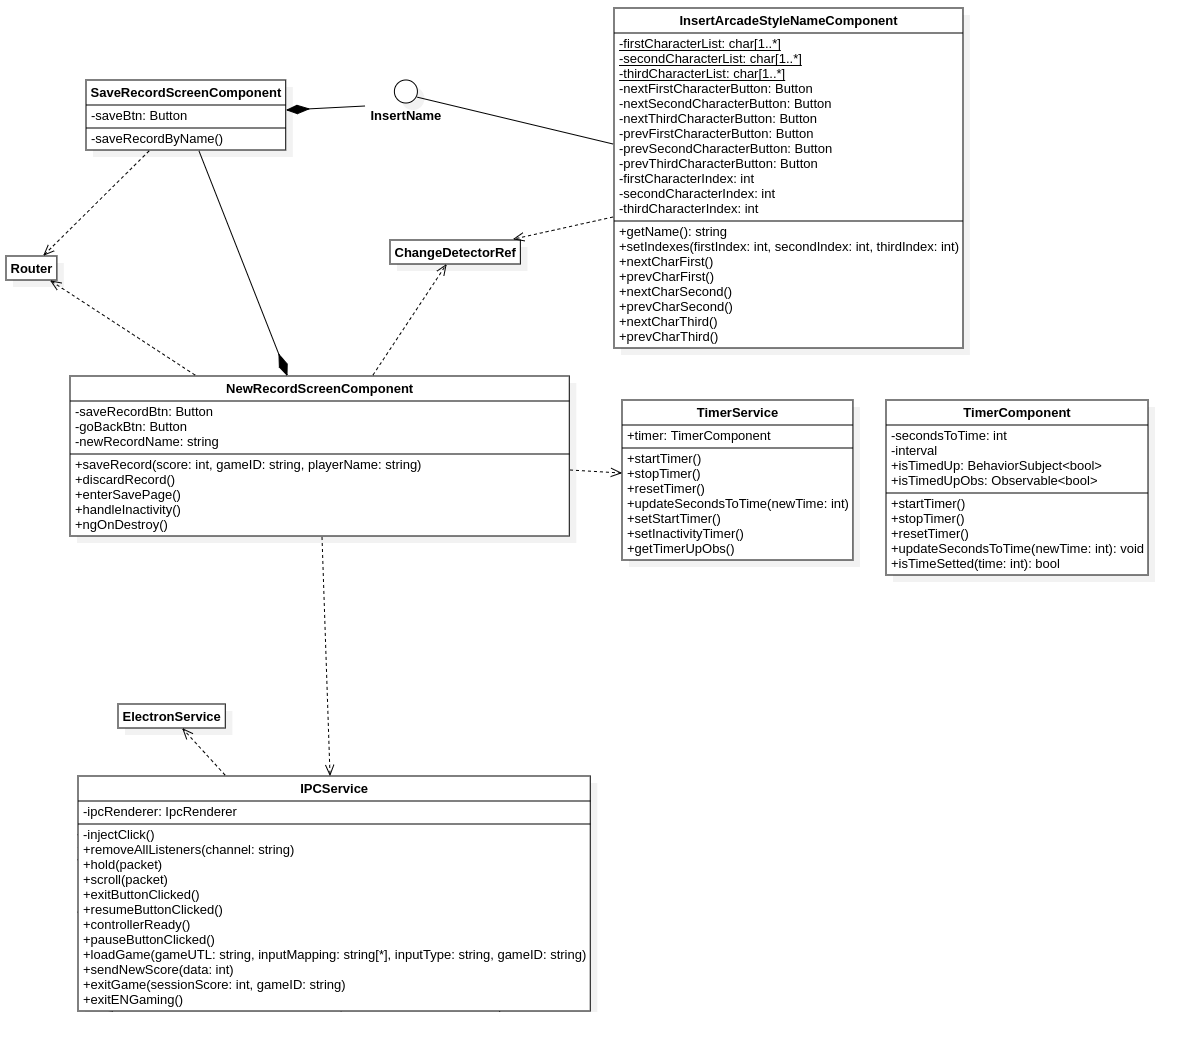
\includegraphics[width=340pt]{images/prog/NewRecord.png}
    \caption{Diagramma delle classi per il salvataggio dei record}
    \label{fig:newRecord}
\end{figure}
% immagine dettaglio salvataggio record
Alla notifica di un nuovo record, viene visualizzata la pagina \emph{NewRecordScreenComponent}, dove viene chiesto all'utente se desidera salvare il record appena effettuato o non salvarlo.\\
Nel caso di salvataggio del record, si passa alla pagina \emph{SaveRecordScreenComponent}, utilizzando un \emph{Router}, che si occupa di ricevere il nome dell'utente. Per far ciò, si avvale della classe \emph{InsertArcadeStyleNameComponent}.\\
Tale classe, che implementa l'interfaccia \emph{InsertName}, prevede l'inserimento dei tre caratteri che compongono il nome utente scegliendo tra i caratteri disponibili, utilizzando gli appositi bottoni.\\
\emph{SaveRecordScreenComponent} inoltre utilizza anche \emph{TimerComponent} attraverso \emph{TimerService} per la gestione dell'inattività in quella determinata schermata.
\newpage
\subsubsection{TimerComponent}
\begin{figure}[h]
    \centering
    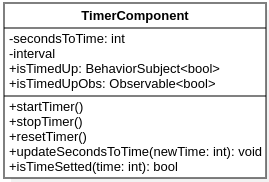
\includegraphics[width=200pt]{images/prog/TimerComponent.png}
    \caption{Dettaglio della classe TimerComponent}
    \label{fig:timer}
\end{figure}
% immagine dettaglio TimerComponent
\emph{TimerComponent}, servito in altri componenti attraverso \emph{TimerService}, si occupa della gestione del tempo.\\ 
Il suo scopo è, dato un tempo espresso in millisecondi, d'iniziare il conteggio, e notificare quando il tempo ha raggiunto la fine.\\
Per far questo, imposta un intervallo della durata memorizzata, notificando tramite un \emph{Observable} quando scade.
\subsubsection{Gestione ENSign11}
\begin{figure}[h]
    \centering
    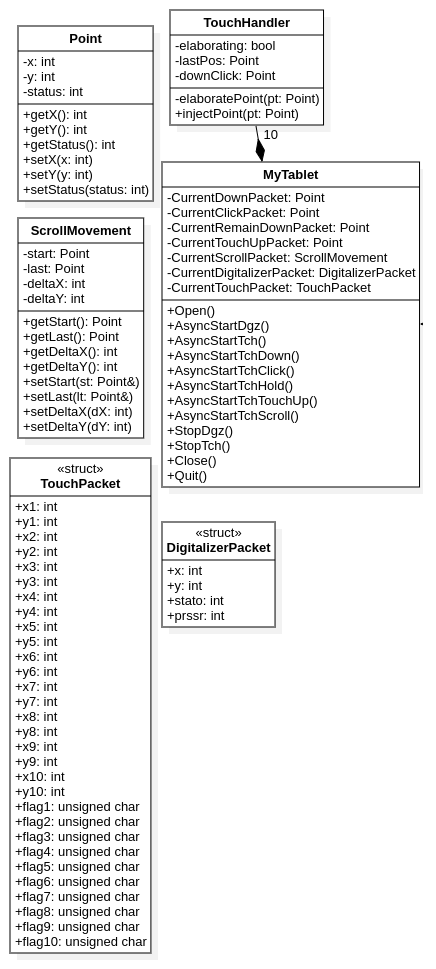
\includegraphics[width=115pt]{images/prog/ENS11.png}
    \caption{Diagramma per la gestione dell'input da ENSign11}
    \label{fig:es11}
\end{figure}
% immagine dettaglio gestione ENSign11
Il device di firma, ovvero l'ENSign11, fornisce le funzioni per interagire con lo stesso attraverso una classe, chiamata \emph{MyTablet}.\\
Questa classe permette l'interazione con il device, come l'apertura e la chiusura dello stesso. Inoltre, offre le funzioni per ottenere gli input dallo stesso.\\
Per il recupero dell'input dal device ENSign11, \emph{MyTablet} si serve della classe \emph{TouchHandler} per il recupero di eventi click, hold, scroll...\\
Questa classe, della quale \emph{MyTablet} ha dieci istanze (una per ogni possibile iterazione, per un massimo di dieci tocchi in contemporanea), rileva se quanto avviene sullo schermo rientra tra i seguenti eventi:
\begin{itemize}
    \item \textbf{Down}: il primo pacchetto che il driver "emette", indica che il dito è stato appena appoggiato sullo schermo.
    \item \textbf{Click}: indica che il dito è stato appoggiato sullo schermo per un breve periodo di tempo.
    \item \textbf{Scroll}: indica che il dito è ancora appoggiato sullo schermo, ma le sue coordinate hanno superato la tolleranza (impostata per evitare falsi movimenti).
    \item \textbf{Hold}: indica che il dito è ancora appoggiato sullo schermo.
    \item \textbf{Touch Up}: l'ultimo pacchetto che il driver "emette", indica che il dito è stato sollevato dallo schermo.
\end{itemize}
I punti, rappresentati da oggetti, che \emph{MyTablet} manda attraverso gli appositi metodi sono:
\begin{itemize}
    \item \textbf{Point}: oggetto che contiene le coordinate del punto e lo stato. Questo oggetto viene mandato per gli eventi elencati prima, a eccezione dell'evento \textbf{Scroll}, durante i giochi che richiedono l'uso del controller e nell'utilizzo generale dell'applicativo.
    \item \textbf{ScrollMovement}: oggetto che contiene i punti (attraverso oggetti \emph{Point}) d'inizio e fine del movimento, e le variazioni delle coordinate x e y. Questo oggetto viene mandato per l'evento \textbf{Scroll}.
    \item \textbf{TouchPacket}: oggetto che contiene le coordinate e lo stato di tutti e dieci i tocchi. L'oggetto viene inviato durante l'esecuzione di giochi che non richiedono l'uso del controller.
    \item \textbf{DigitalizerPacket}: oggetto che contiene le coordinate, lo stato del digitalizer e la pressione applicata dall'utente. L'oggetto viene inviato durante l'esecuzione di giochi che non richiedono l'uso del controller.
\end{itemize}
\subsubsection{Servizi di Angular}
\label{subsec:angularServices}
ENGaming utilizza i seguenti servizi, offerti da Angular, per l'esecuzione del programma:
\begin{itemize}
    \item \textbf{Router}: permette di essere reindirizzati da un componente a un altro, aggiornando la vista, tramite il metodo \emph{navigate}.
    \item \textbf{ChangeDetectorRef}: aggiorna la vista tramite il metodo \emph{detectChanges}.
    \item \textbf{ActivatedRoute}: permette di recuperare l'URL della pagina in cui ci si trova.
    \item \textbf{ElectronService}: permette l'utilizzo dei canali IPC e delle funzioni generalmente presenti in Electron.
    \item \textbf{DomSanitizer}: effettua il processo di "pulizia" di un URL, permettendo la visualizzazione del suo contenuto in un elemento \emph{iframe} oppure \emph{object}.
\end{itemize}
\subsection{Struttura dei file utilizzati}
\label{subsec:strutturaFile}
Come indicato in \nameref{subsec:gameComponent} e \nameref{subsec:recordComponent}, vengono utilizzati due file json, il primo contiene le informazioni sui giochi (\emph{games.json}), il secondo contiene i record effettuati (\emph{records.json}).
\subsubsection{Games.json}
Il file, che viene aperto da ENGaming solamente in lettura, contiene le informazioni necessarie dei giochi e delle loro relative pagine. Ne consegue che la modifica di questo file debba essere fatta manualmente.\\
Un esempio di giochi presenti nel file è il seguente:
\begin{lstlisting}[language=json,firstnumber=1]
    [
        {
            "id": "catMario",
            "name": "Cat Mario",
            "type": "Azione",
            "gameURL": "https://www.cat-mario.com/",
            "inputType": "controller",
            "description": "Clone di Super Mario, con un gatto. Per nulla stressante!",
            "inputMapping": [
                "salto:A:Space",
                "muovi a sinistra:DPad Left:Left",
                "muovi a destra:DPad Right:Right"
            ]
        },
        {
            "id": "subwaySurfers",
            "name": "Subway Surfers",
            "type": "Endless",
            "gameURL": "src_angular/assets/games/subwaySurfers/index.html",
            "inputType": "touchDigit",
            "description": "not_available",
            "inputMapping": [
                "inizia: tap",
                "muovi a sinistra: swipe a sinistra",
                "muovi a destra: swipe a destra",
                "salto: swipe in alto",
                "rotolata:swipe in basso"
            ]
        }
    ]
\end{lstlisting}
Dove i giochi con il controller richiedono anche la conoscenza dei tasti che il gioco richiede tramite l'utilizzo della tastiera.\\
Inoltre, i giochi possono essere caricati con i sorgenti tramite il percorso relativo degli stessi.
\newpage
\subsubsection{Records.json}
Il file contiene tutti i record effettuati nell'applicativo. Tale file non è condiviso in rete ed è unico per ogni installazione. Quindi, i record possono variare da una macchina a un'altra.\\
Questo è l'unico file che viene caricato da ENGaming sia per la lettura che per la scrittura, non richiedendo una scrittura manuale dei dati.\\
Un esempio di record che il file contiene è il seguente:
\begin{lstlisting}[language=json,firstnumber=1]
    [
        {
            "userName": "AAA",
            "score": "250",
            "gameID": "dukeNukem",
            "dateTime":"2024-02-15 17:23"
        },
        {
            "userName": "RIC",
            "score": "420",
            "gameID": "angryBirds",
            "dateTime":"2024-05-19 08:23"
        }
    ]
\end{lstlisting}
\subsection{Scelte progettuali}
Oltre a quanto già visto, ho adoperato diverse scelte durante questa fase.\\
In particolare:
\begin{itemize}
    \item architetturalmente, ho scelto di utilizzare il modello Model-View-ViewModel (abbreviato MVVM), in quanto tra le possibili architetture l'ho ritenuta la più adatta per il progetto.
    \item l'utilizzo di \Gls{angl} mi consente di ridurre l'accoppiamento per componenti attraverso l'utilizzo della \emph{Dependency Injection} per l'utilizzo dei servizi.
    \item l'utilizzo degli \Gls{ipcg} mi permettono di far comunicare gli elementi che compongono l'applicazione, in particolare tra le classi implementate in \Gls{angl} ed \Gls{elctr}, attraverso lo scambio di messaggi in appositi canali.\\Tale comportamento è simile al comportamento di un \emph{Observer}.
    \item per rendere minore la dipendenza tra le componenti, ho scelto di non utilizzare alcun tipo di gerarchia. Questa scelta è dovuta, oltre alla non reale necessità del suo utilizzo, alla limitatezza a livello applicativo, in quanto tra le tecnologie da usare solo \gls{cpp} permette l'uso di una gerarchia.
    \item invece di ricorrere all'utilizzo delle gerarchie, ho scelto di definire le parti comuni attraverso un'interfaccia, che viene poi implementata dalle singole classi che la necessitano.
\end{itemize}
\section{Codifica}
\minput{Prodotto/sviluppo}
\minput{Prodotto/prodotto}